\chapter{Technical Design}

This chapter will give a overview of the structure of the application as well as some choices taken when developing the research product, Nevrolens. The chapter will exclusively focus on the application as it is at the end of this research project, which is functionally identical to version 0.3.3 of Nevrolens. However, some refactoring i.e. name changes and restructuring may have occurred. 

\section{Game Structure}

\subsection*{Unity Scene Graph}

Within Unity a \textit{Scene} consists of a \textit{scene graph} which is a tree structure of \texttt{GameObjects}. By default a scene consist of a \texttt{Directional Light} lighting up the scene at its default light source and a \texttt{Main Camera} which is the view point of the running game. In addition, the MRTK library will add two objects to the scene graph, one called \texttt{MixedRealityToolkit} which contains configuration of the Mixed Reality features and systems. This is where input systems are defined and where control of spatial awareness and boundary detection is handled, in short all features and sensors of the HoloLens system or other AR system are defined and controlled here. The other object added by MRTK is the \texttt{MixedRealityPlayspace}, this encapsulates the \texttt{Main Camera}, but is lacking any useful documentation on what its purpose is. The name could be hinting at it being the parent of the \textit{Playspace}, meaning all \texttt{GameObjects} in the game. However, even MRTK demos seem to ignore this object and thus it has not been used in this project either.

The functionality of the scene graph, other than organizing GameObjects, is that child objects inherit the position, rotation and scale of their parents, thus simplifying transformation of complex object. This naturally structures many systems, however in a AR application there can be many independent 3D objects floating in space. In addition, some objects are dependent not on their parent, but on a defined object \texttt{Transform}. Therefore, some organization is needed and some objects are placed by choice and convenience rather than any practical reason. Another practical use for child objects are the use of the \texttt{GameObject.GetComponentsInChildren()} and \texttt{GameObject.GetComponentInParent()} methods which allows for simple access to \texttt{Components} in child and parent \texttt{GameObjects}, this is however of limited use as such dependencies in code has a tendency to result in tedious bugs.

The top most application specific object of the project is the \texttt{BrainSystem}, this acts as the parent GameObject for all objects defined by the application. The right side of \autoref{fig:brainsystem} gives an overview of all 3D object in the \texttt{BrainSystem}. The \texttt{InfoBoard} on the right, the button group, or \texttt{HandMenu} in the center and the complete brain model with axes etc. named \texttt{GameWorldSpace}, are spatially independent systems all having \texttt{BrainSystem} as a parent, this can also be seen in \autoref{fig:brainsystem} in the scene hierarchy on the left side. The reasoning for having the parent object \texttt{BrainSystem} is purely to to tidy up the top layer of the scene graph and having a clear distinction of project specific custom objects. 

The main attraction within the \texttt{BrainSystem} is the \texttt{GameWorldSpace}, it is the parent of the brain model and all objects with are spatially dependent on the brain. This allows for movement and scaling of the whole model worldspace. This is also the local space of the synchronized multiplayer world. 

% notice that the blue "black board" on the right, the button group and the brain are independent spatially.

\begin{figure}[ht]
    \centering
    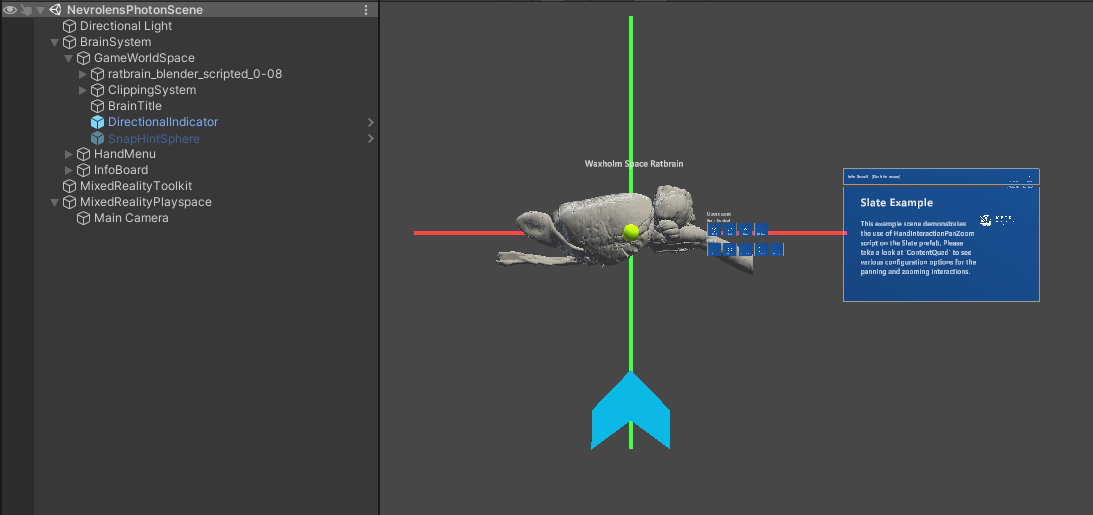
\includegraphics[width=\textwidth]{fig/brainsystemoverview5.png}
    \caption{Every 3D object in the \texttt{BrainSystem}}
    \label{fig:brainsystem}
\end{figure}
% In general there is few limitations on how to structure the scene graph, its functionality other than structural,

\section{Networking}

\subsection*{Networking Solutions}

Multiplayer games in Unity can be created in numerous ways, in the development phase of this project three solutions were explored; UNET,  LiteNetLib and Photon PUN2 . Common for all are that they are mature, reliable and are well documented, they all support multiple device types including all devices within the scope of this project, there are however some very clear differences making the choice for this project quite simple.
% mlapi, mirror, playfab
\textit{UNET} is Unity's own default networking solution, it provides high level functionality and is generally easy to use. It is however deprecated and will be discontinued by the end of 2021, an open source fork of the networking API, called \textit{Mirror} has seen continuing development and improvement, but because of the state of the original project, both were deemed nonideal. Unity is working on a new networking solution called \textit{MLAPI}, it is in alpha stages but shows great promise.

\textit{LiteNetLib} is a open source, and more low level framework. It is intended for use cases where in-depth control of the networking processer are wanted or needed, if high performance and low latency is important this would be a good choice. It supports peer-to-peer and self-managed servers. Because this project can be thought of a small scale proof of concept, it is of limited concern whether the networking is highly performant and seeing as a low level API is more complicated to implement it is neither a optimal use of a single developers time.

Lastly, \textit{Photon PUN2} is the an high level networking library with managed hosting and a free basic plan for up till 20 concurrent users. This makes it ideal for small projects and single developers. It is also the general first choice for networking solution in Unity and its surge in popularity is partly the reason for Unity abandoning their own solution. PUN2 was a natural choice simply because is of its low barrier for entry and it having a free hosting options making development as easy as possible. It being the most popular solution also has the added benefit of having well made tutorials and forums for troubleshooting.

While developing this application, Microsoft announced a new solution for networking specifically targeting MR applications called \textit{Microsoft Mesh}, it promises to solve networking, and many MR specific problems like spatial anchoring and face-to-face interaction. This could be a promising step for this application in the projects continuation, and should be kept an eye on by future researchers.

\subsection*{Networking Design}

\begin{wrapfigure}[14]{r}{0.4\textwidth} 
    \centering
    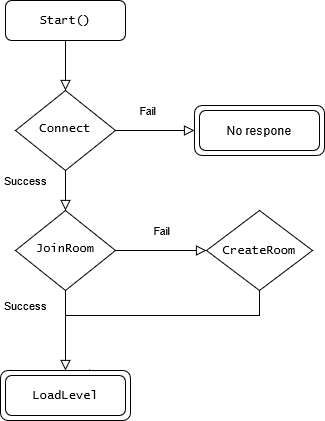
\includegraphics[width=0.3\textwidth]{fig/photonconnectiondiagram2.png}
    \caption{State diagram of the implemented connection process}
    \vspace{30pt}
    \label{fig:photonconnect}
\end{wrapfigure}
In this project, networking has as stated been implemented as simply as possible for a proof of concept and because of time constraints on a single developer. If concerns like scalability and reliability was of higher importance different choices would have been made, and steps to fulfill those concerns should probably be taken in future development.
When using the networking, which is how the built versions of the application are set up, the application initially launches in a empty \texttt{Scene} named \texttt{NevrolensStartPhotonScene}, its only purpose is connecting the user to the server and creating or joining a \textit{room}. A room is a Photon abstraction for connecting users to the same game state. \autoref{item:photonconnect} shows a striped down version of the script running in this scene, it is a complete and functional script to emphasize the ease of implementation. The script  is all that is needed to initiate a connation in Photon PUN2, and is all connection handling in the application. The implementation has, because of its simplicity, some flaws, \autoref{fig:photonconnect} shows that if connection to the photon server fails the application will give no response and the user will just stay in an empty scene, this could easily be fixed by either giving some error message feedback with a retry button or even loading the game scene in offline mode, neither has been implement mainly because connation issues have seldom raised and thus development time has not been invested in fixing this problem. 

\begin{lstlisting}[language=c, label={item:photonconnect}, caption={The connect process in a Unity \texttt{MonoBehaviour} written in C\#. }]
    void Start() {
        PhotonNetwork.ConnectUsingSettings();
    }
    override void OnConnectedToMaster() {
        PhotonNetwork.JoinRandomRoom(); 
    }
    override void OnJoinRandomFailed(short returnCode, string msg) {
        PhotonNetwork.CreateRoom(roomName: "room1"); 
    }
    override void OnJoinedRoom() {
        if (PhotonNetwork.IsMasterClient)
            PhotonNetwork.LoadLevel("NevrolensPhotonScene");
    }
\end{lstlisting}

Another implication of this design is that every user will necessarily connect to the same room. This happens because the first user will find no room and thus create a new one, while all others will find the one room and connect to it. The user has no control over who they play with, and can not start a session by them self, both could easily be implemented, but would also result in overhead for the user as they will have to make a choice which now is simply made for them.

All in all this solution work well enough for the current state of the research project. In fact, by abstracting away the connection and room selection process it has simplified the user testing process because there are fewer steps to get to a running application. 



